\documentclass[a4paper]{article}

%% Language and font encodings
\usepackage[french]{babel}
\usepackage[utf8x]{inputenc}
\usepackage[T1]{fontenc}
\usepackage{wrapfig}

%% Sets page size and margins
\usepackage[a4paper,top=3cm,bottom=2cm,left=3cm,right=3cm,marginparwidth=1.75cm]{geometry}

%% Useful packages
\usepackage{amsmath}
\usepackage{pdfpages}
\usepackage{graphicx}
\usepackage[colorinlistoftodos]{todonotes}
\usepackage[colorlinks=true, allcolors=blue, breaklinks=true]{hyperref}

\newcommand{\guill}[1]{\og{}#1\fg{}}

\title{Le planning de ma cuisine}
\author{Adrien Krähenbühl \and Basile Sauvage \and Julien Narboux}
\date{2018}

\begin{document}
\maketitle

\begin{abstract}
Description d'une activité d'informatique débranchée sur le thème de l'ordonnancement.
\end{abstract}

\smallskip

\textbf{Mots clés:} algorithme, ordonnancement, complexité, Johnson, informatique débranchée, cs-unplugged

\section{Description du jeu}

On se trouve dans une cuisine avec un ensemble de plats à préparer qui nécessitent chacun un certain temps de préparation et un certain temps de cuisson. Le cuisinier ou la cuisinière ne peut préparer qu'un seul plat à la fois, et le four ne peut accueillir qu'un plat à la fois.

L'objectif est de trouver l'ordre de préparation des plats qui permet de terminer l'ensemble de tous les plats le plus rapidement possible.

\section{Matériel}

La matériel consiste en la matérialisation d'un diagramme permettant de réprésenter la plannification des tâches (ce genre de diagramme est appelé diagramme de Gantt).

Les temps de cuisson et de préparation des plats sont matérialisés par des rectangles de longueur proportionelle à la durée. Les temps de préparation sont indiqués par une toque, les temps de cuisson par un four.

Le matériel peut être construit en bois pour une utilisation intensive ou simplement en papier pour une activité en classe, des patrons sont fournis en annexe.

Le montage que nous avons réalisé consiste en une baguette de 67mm de large, trois baguettes de 9mmx9mm qui servent de guide et des rectangles découpés dans des baquettes de 18mm de large ce qu'il laisse 67-3*9-2*18=4mm de marge pour que les baguettes coulissent facilement. A refaire, il vaudrait mieux avoir une largeur différente pour les temps de préparation et les temps de cuisson, comme çà les participants ne peuvent pas se tromper.

Le meilleur temps possible pour chaque défi est indiqué par une marque sur une règle donnant l'échelle de temps.

Toutes les sources sont disponibles ici:
\url{https://github.com/jnarboux/MediationInfoStrasbourg/tree/master/ordonnancement}

Les commentaires et suggestions d'améliorations sont les bienvenus.

\begin{figure}
\begin{center}
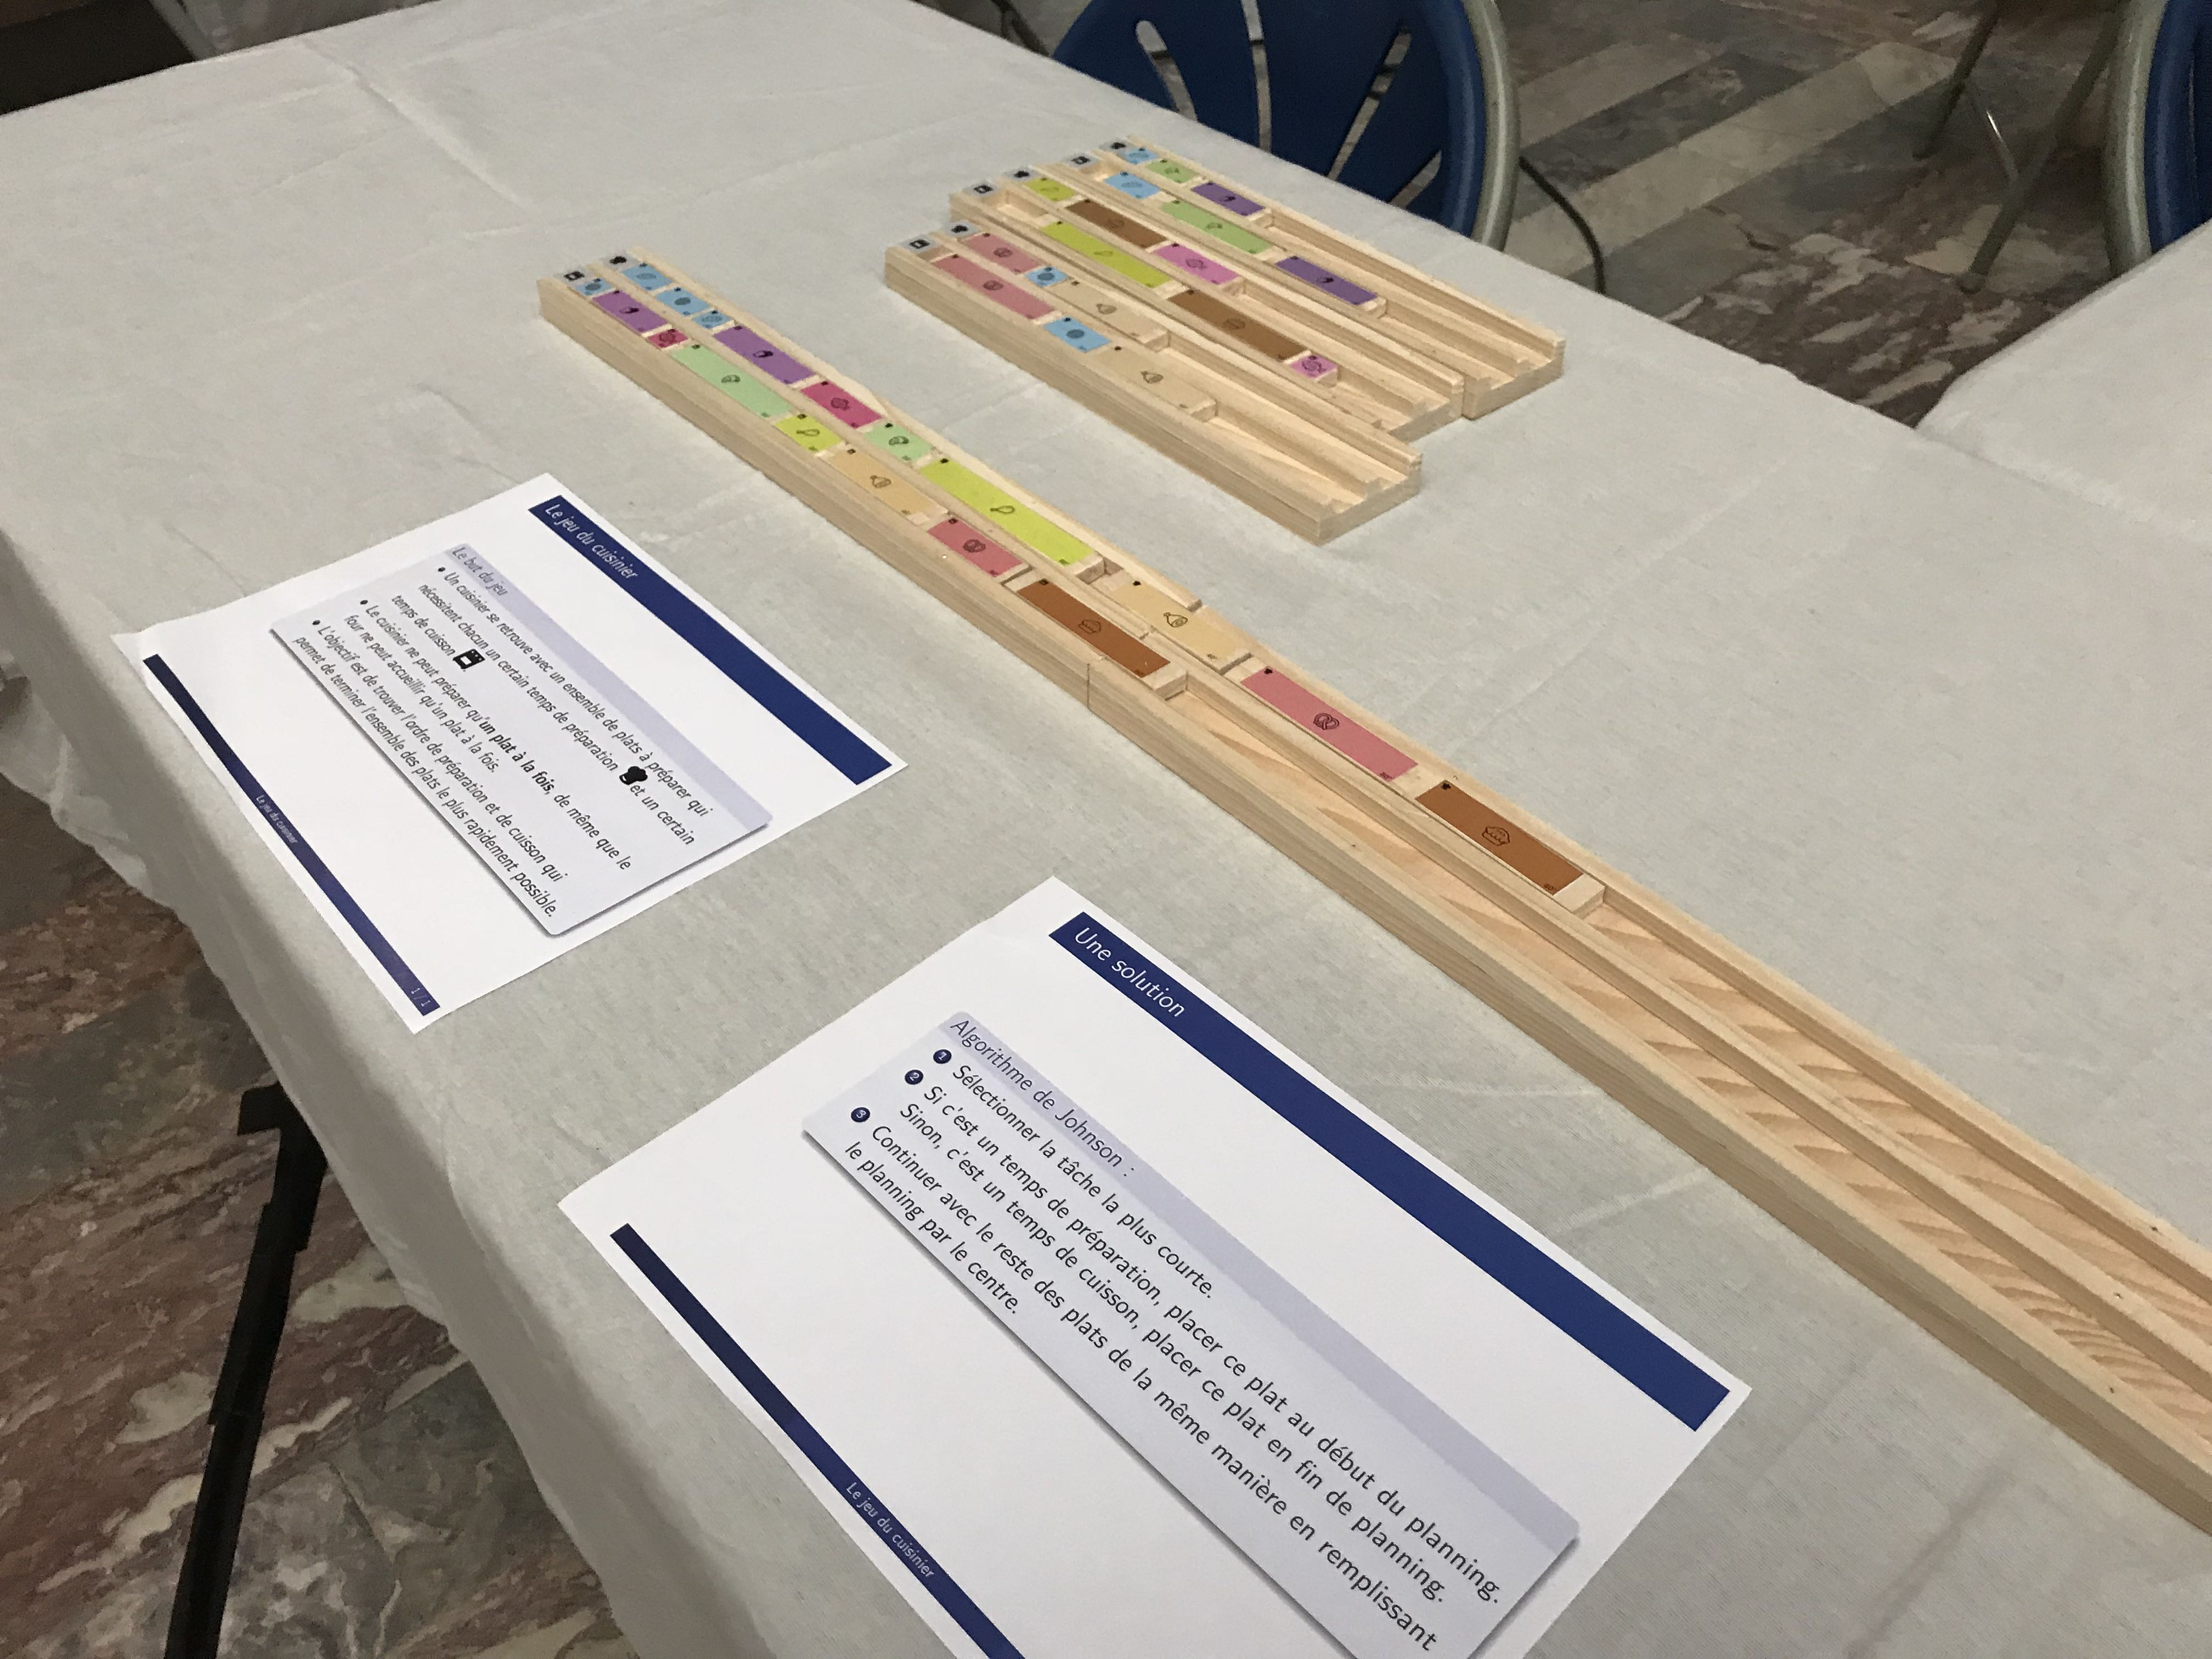
\includegraphics[width=0.8\textwidth]{photo_materiel.jpg}
\end{center}
\caption{Le matériel.}
\end{figure}

\section{Déroulement de l'activité}

Nous proposons quatre défis et quelques questions et explications:
\begin{enumerate}
\item On explique les règles du jeu sur un exemple en choisissant un ordonnacement pas optimal.
\item Un premier défi (le boulanger: croissant, brioche, pain). On laisse le joueur essayer, une solution est vite trouvée. On peut alors demander ``Quelle méthode avez-vous utilisée ?'', `'Est-ce que c'est la meilleure solution?''
Sur cet exemple, si on trie les plats par ordre de temps de préparation croissant, on obtient une solution optimale. 
\item Un deuxième défi (le restau alsacien: tarte flambée, jambonneau, bretzel) montre que trier par temps de préparation croissant n'est pas toujours optimal, mais si on trie par temps de cuisson décroissant cela fonctionne sur cet exemple.
\item Un troisième défi (poulet, gâteau, poisson) dont la solution optimale n'est ni un tri croissant des temps de préparation, ni un tri décroissant des temps de cuisson.
\item Un quatrième défi (avec les 9 plats) permet de faire chercher un peu plus les participants, il devient difficile de savoir si l'on a obtenu la solution optimale.
\item On peut alors demander combien il y a d'ordonnancements des 9 plats possibles.
\item On explique l'algorithme de Johnson et on commence à l'éxecuter sur l'exemple.
\item On peut éventuellement poser la question de la complexité de l'algorithme.
\item A la fin on peut ouvrir en expliquant ce qu'est un algorithme, citer quelques applications et parler de problèmes NP-Complets 
\end{enumerate}

\section{Contexte scientifique}


Le problème présenté dans cette activité est un exemple des problèmes étudiés en recherche opérationnelle. Il s'agit de l'étude des méthodes rationnelles pour réaliser une tâche de manière optimale. En particulier la recherche opérationnelle étudie les problèmes dit combinatoires, où il faut choisir parmi un grand nombre de solutions (ordonnancement, gestion de stocks, affectation de ressources, \ldots ).

Le problème présenté ici est connu comme le problème de Johnson, c'est un des premiers problèmes d'ordonnancement étudié. Johnson a proposé une solution quand les plats nécessitent deux tâches~\cite{johnson1954optimal}.

On peut l'exprimer de la manière suivante:
\begin{enumerate}
\item Sélectionner la tâche la plus courte.
\item Si c'est un temps de préparation, placer ce plat au début du planning. Sinon, c'est un temps de cuisson, placer ce plat en fin de planning.
\item Continuer avec le reste des plats de la même manière en remplissant le planning par le centre.
\end{enumerate}

ou bien de la manière suivante:
\begin{enumerate}
\item Séparer les plats en deux catégories: ceux qui sont plus rapides à préparer qu'à cuire (R), et les autres (C).
\item Ordonnancer les plats rapides (R) par temps de préparation croissant, puis les autres par temps de cuisson décroissant. 
\end{enumerate}

%\subsection{Permutations ?}
%
%On peut se poser la question de savoir si on peut toujours trouver une solution optimale en mettant les tâches dans le même ordre dans le four que l'ordre de la préparation.
%
%Généralisons pour des plats qui nécessitent pas deux mais quatre étapes:\\
%\begin{tabular}{lll}
%          &   & \\
%laver  & 1 & 4 \\  
%éplucheur    & 4 & 1 \\
%mixeur & 4 & 1 \\
%cuisson      & 1 & 4 \\
%\end{tabular}

%\subsection{Extensions}

Le problème devient NP-Difficie si on ajoute une troisième machine~\cite{baker2013principles}. En pratique, les problèmes d'ordonnancement sont difficiles, des instances du problèmes avec 15 plats utilisant 15 machines ne sont pas résolues\footnote{Voir \url{https://educnet.enpc.fr/file.php/297/CoursROPonts.pdf}, page 106.}.



\section{Retour d'expérience}

Cette activité a été testée avec le public d'un Village des Sciences en 2018. Le public a été assez attiré par l'installation. Les gens n'ont pas eu de mal à comprendre les règles. Les enfants à partir de 7-8 ans parviennent à résoudre les défis. Certains comparaient l'activité au planning des lessives du week-end: couleur/blanc/laine avec lavage et séchage dans deux machines différentes. 

\begin{figure}[h!]
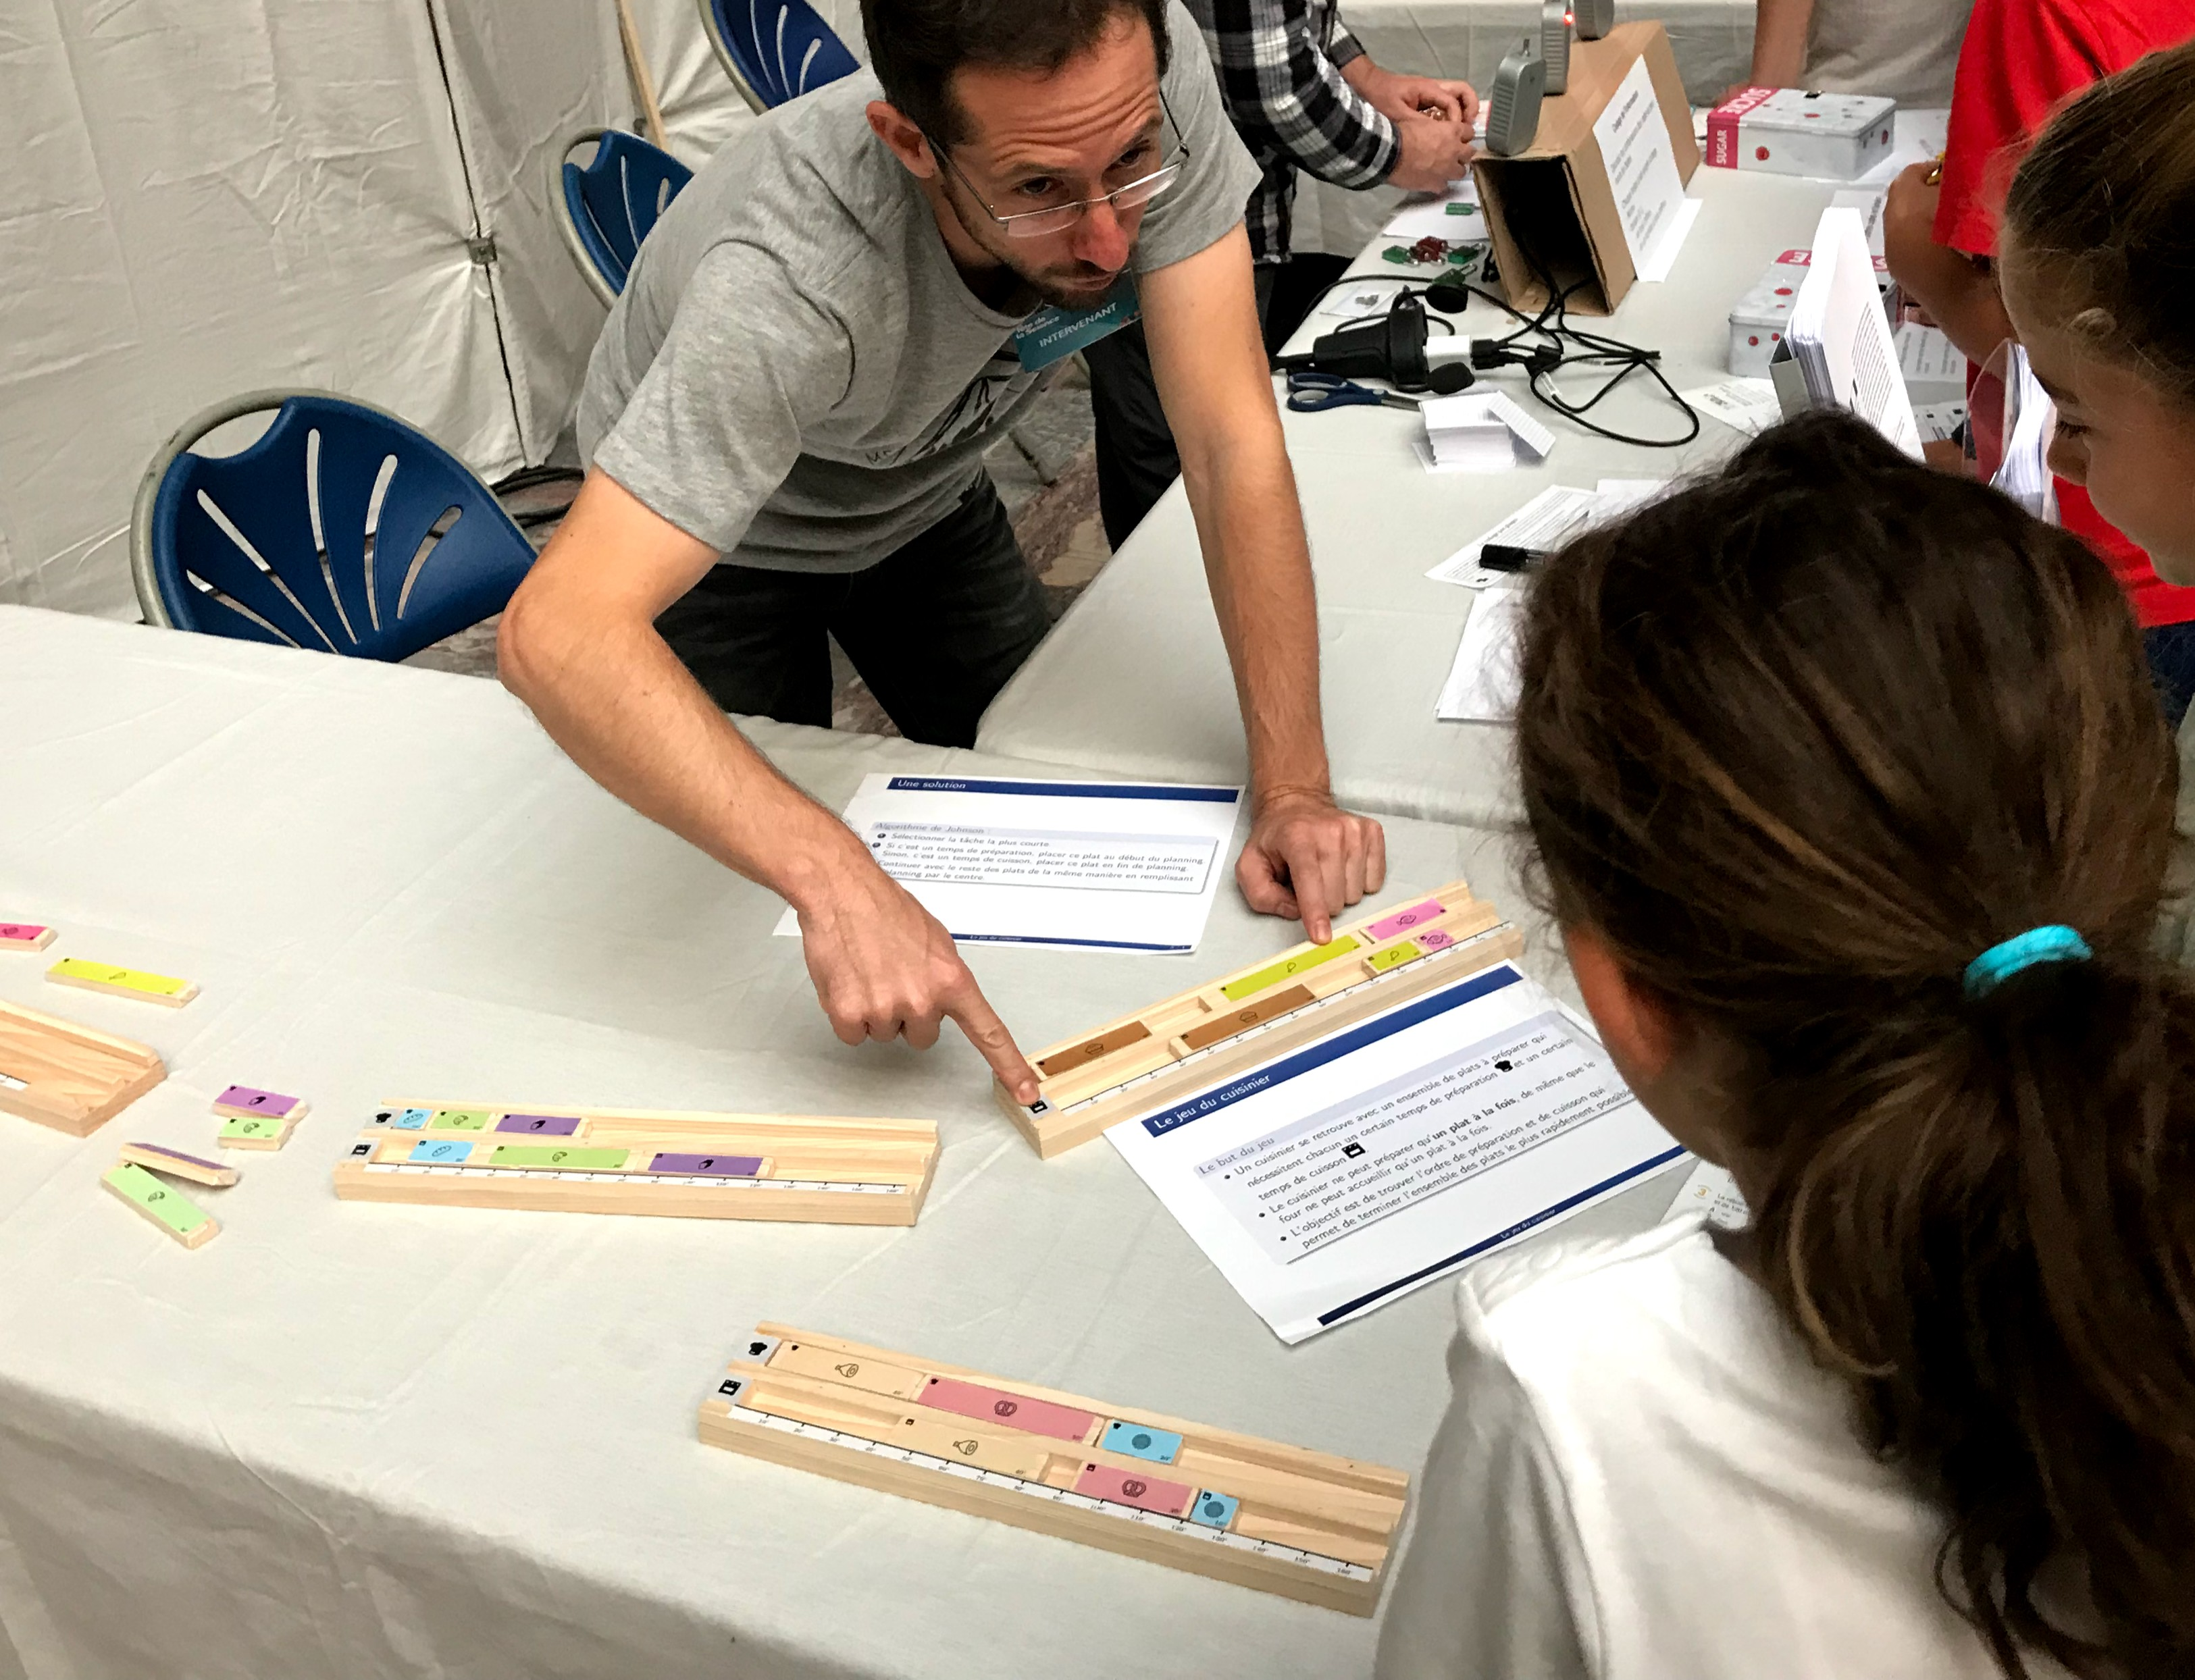
\includegraphics[width=\textwidth]{photo_activite.jpg}\\
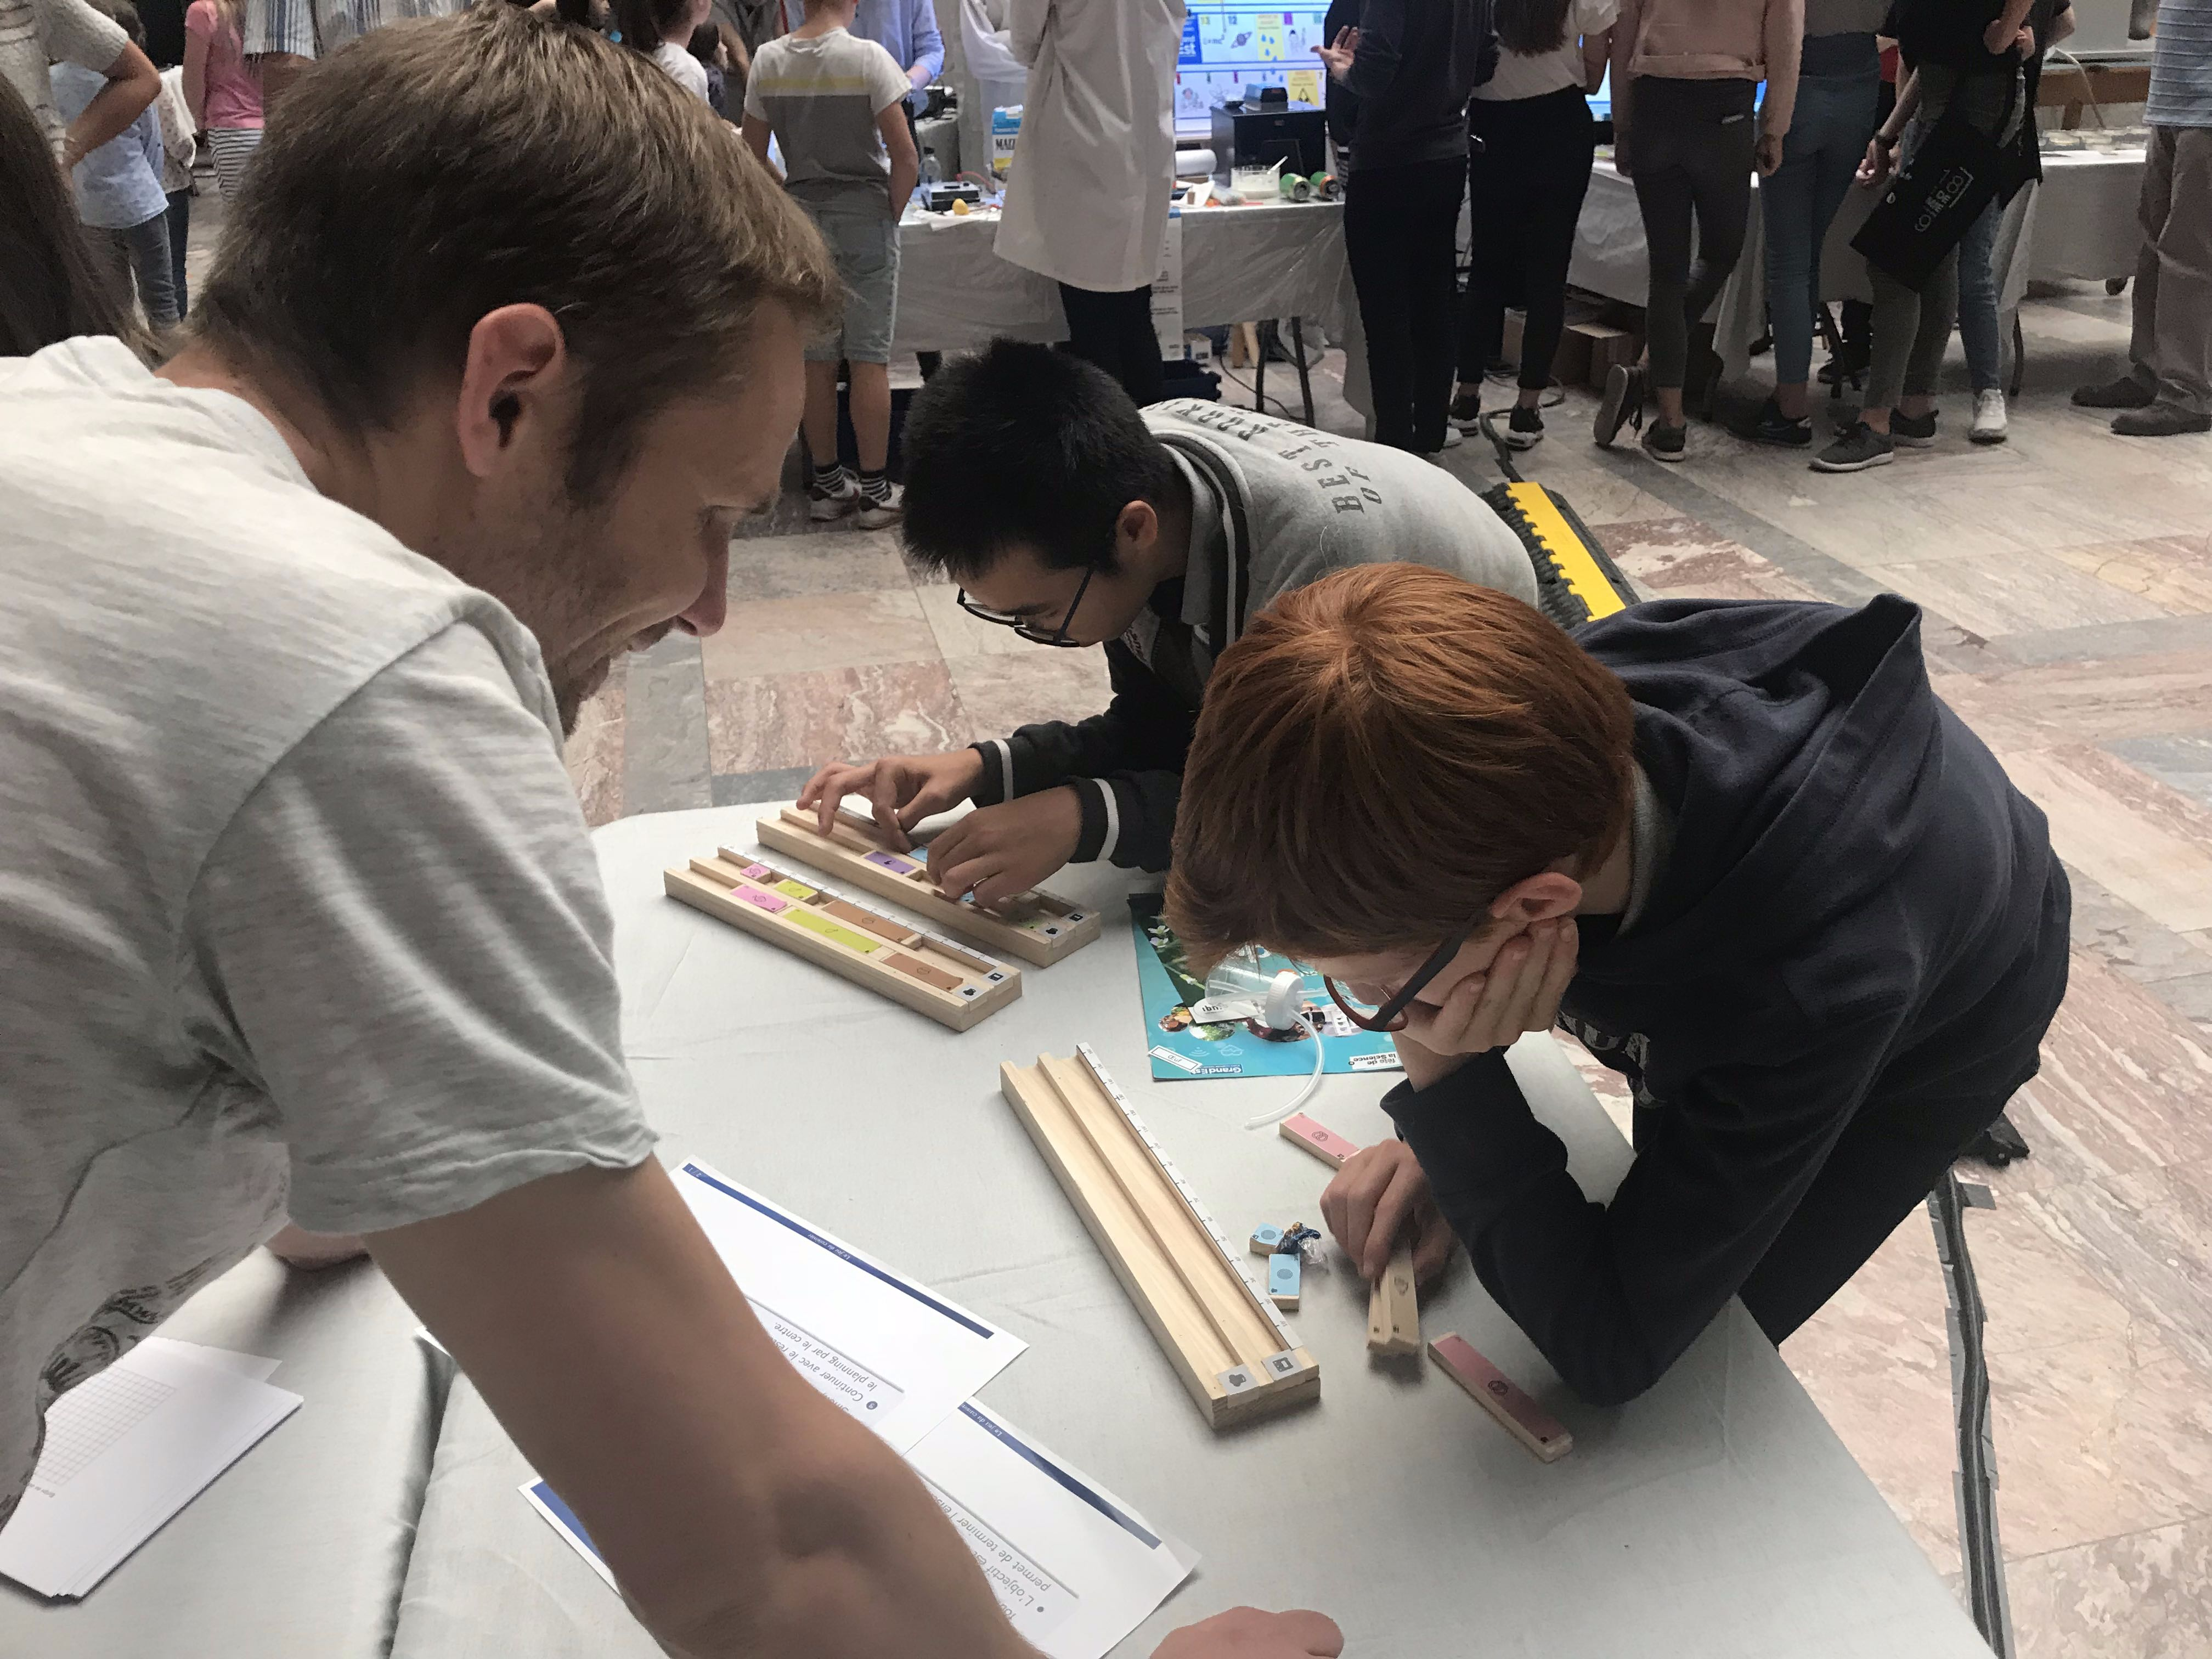
\includegraphics[width=\textwidth]{photo_activite2.jpg}

\caption{Fête de la Science 2018, Strasbourg}
\end{figure}

\section{Pistes d'extensions}

On pourrait envisager d'ajouter à cette activité une deuxième étape avec des graphes de dépendances entre tâches.



\bibliographystyle{alpha}
\bibliography{biblio}


\clearpage

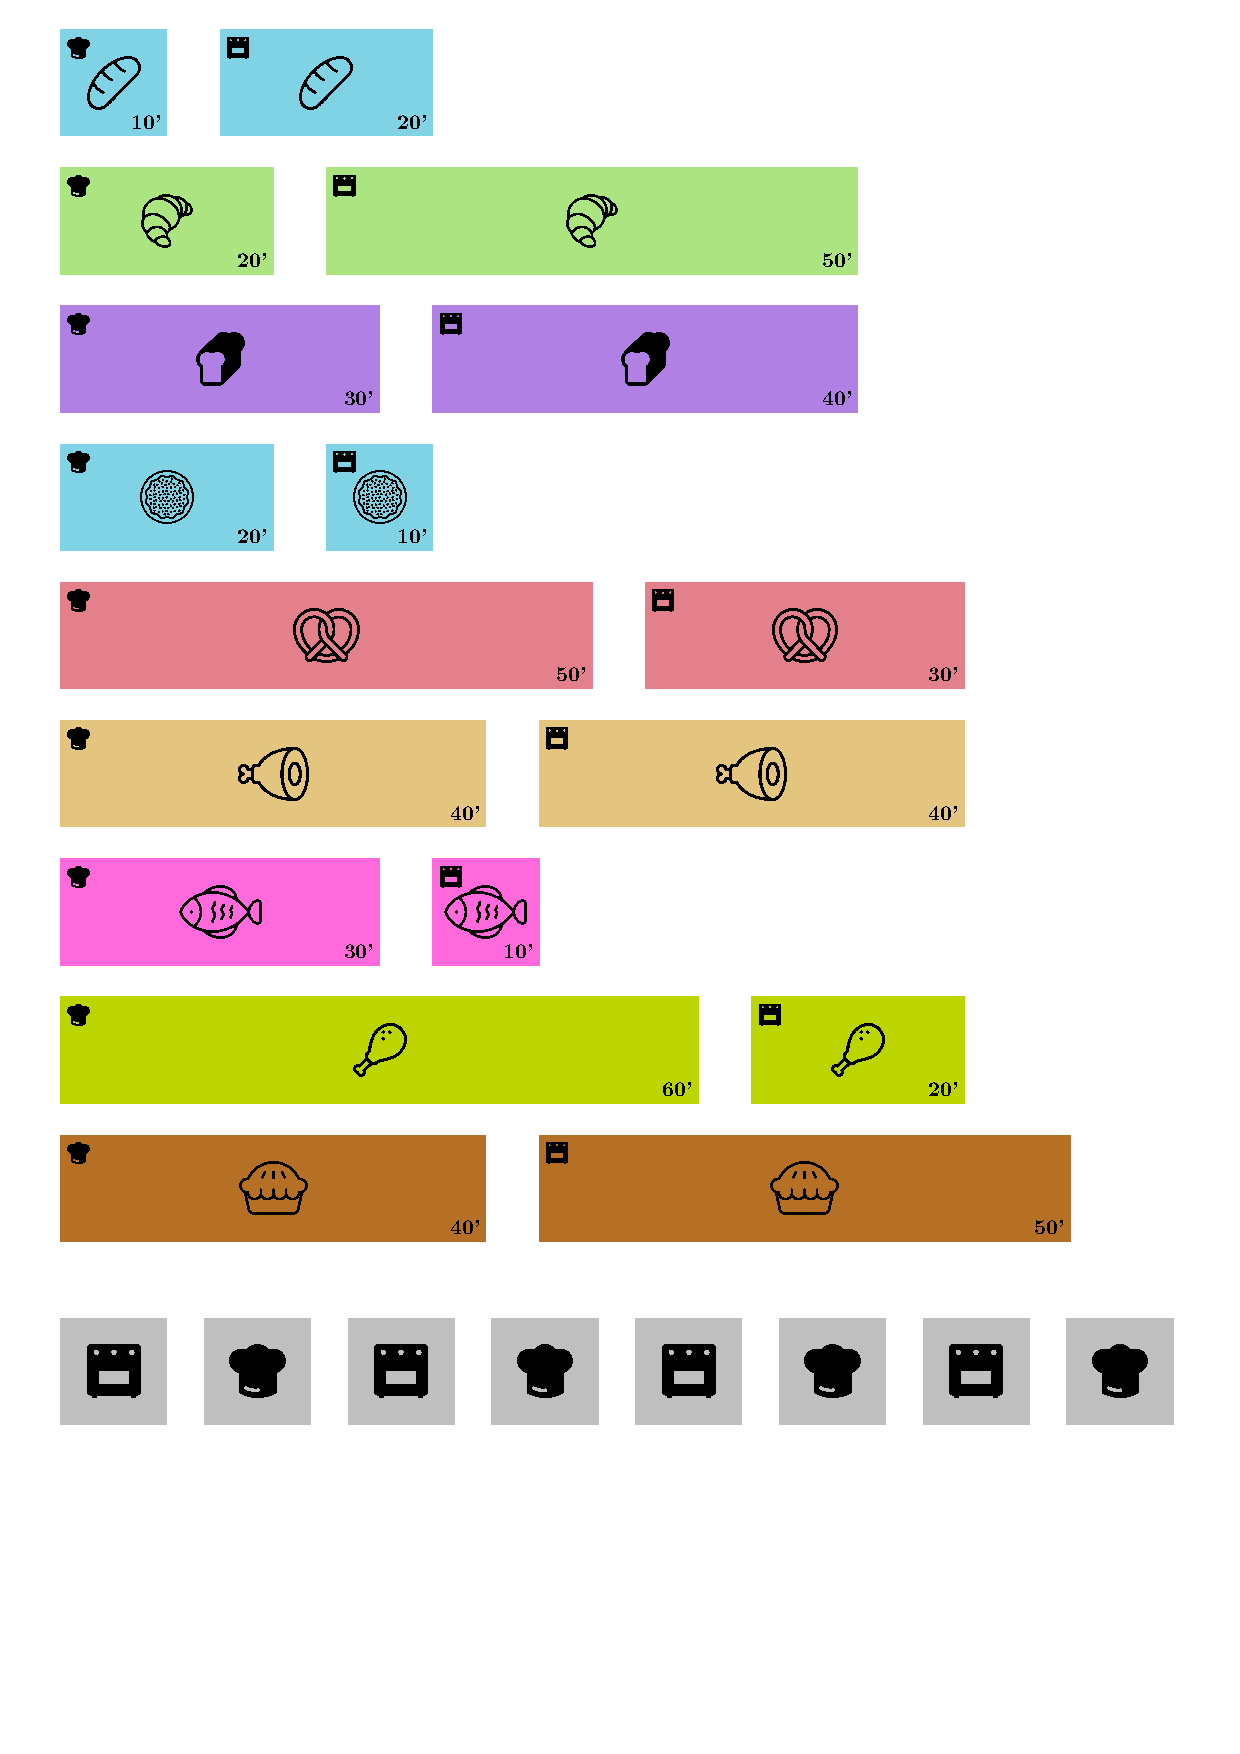
\includepdf{modeles.pdf} 
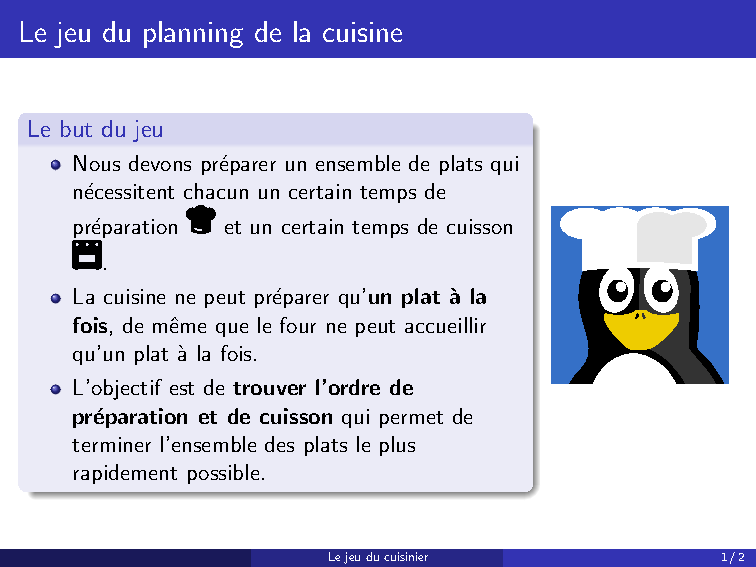
\includepdf[landscape=true,pages=1-2]{explications.pdf}


\end{document}